\documentclass{beamer}
\usetheme{CambridgeUS}

% Title page details:
\title{GoTalk}
\author{Swasti \and Shreya \and Krishika \and Samriddhi}
\date{\today}

\begin{document}

\begin{frame}
    \titlepage
    \centering HACKTIVISTS
\end{frame}

\begin{frame}{PROJECT AIM}
    To develop a real-time chat web application with chat history retrieval using Go, WebSocket and Firebase majorly.   
    \\
    Our main aim is to Learn the Go language and Firebase and learn how to establish a client-server connection using WebSocket .
\end{frame}

\section{Tech Stack}
\begin{frame}{Tech Stack}
    \begin{itemize}
        \item \textbf{Frontend}
        \begin{itemize}
            \item HTML/CSS
            \item JavaScript
            \item Bootstrap/Tailwind CSS
        \end{itemize}
        \item \textbf{Backend}
        \begin{itemize}
            \item Go (Golang)
            \item Gorilla WebSocket
            \item Firebase Realtime Database
        \end{itemize}
    \end{itemize}
\end{frame}

\section{Tasks Completed Till Now}

\begin{frame}{Tasks Completed Till Now}
    \begin{itemize}
        \item \textbf{Initial Setup:}
        \begin{itemize}
            \item Set up Go development environment.
            \item Created basic Go app with WebSocket support.
        \end{itemize}
        \item \textbf{Firebase Integration:}
        \begin{itemize}
            \item Set up Firebase Realtime Database for chat data storage.
        \end{itemize}
    \end{itemize}
\end{frame}

\begin{frame}{Tasks Completed Till Now (Contd.)}
    \begin{itemize}
        \item \textbf{Bidirectional Communication:}
        \begin{itemize}
            \item Implemented WebSocket-based communication.
            \item Established real-time messaging.
        \end{itemize}
        \item \textbf{Past Chat Retrieval:}
        \begin{itemize}
            \item Retrieved past chats from Firebase.
            \item Displaying past chats.
        \end{itemize}
    \end{itemize}
\end{frame}

\begin{frame}{Tasks Completed Till Now (Contd.)}
    \begin{itemize}
        \item \textbf{Basic UI Development:}
        \begin{itemize}
            \item Added basic styles for chat interface.
            \item Created simple layout for message display.
        \end{itemize}
    \end{itemize}
\end{frame}

\section{New Tasks Done}

\begin{frame}{Tasks done after the last progress presentation (10.07.24)}
    \textbf{This was to be shown on Friday, 12.07.2024}
    \begin{itemize}
        \item \textbf{Rooms Functionality:}
        \begin{itemize}
            \item Implemented separate chat rooms.
            \item Created three distinct chat rooms.
            \item Ensured message isolation per room.
        \end{itemize}
        \item \textbf{Enhanced UI:}
        \begin{itemize}
            \item Improved chat interface design.
            \item Added user-friendly styles.
        \end{itemize}
    \end{itemize}
\end{frame}

\section{Tasks done so far}

\begin{frame}{Tasks achieved during 13-15th July, 2024:}
    \textbf{Cookie Implementation:}
        \begin{itemize}
            \item Implement cookies for session management.
            \item Ensure that on reloading the application doesn't prompt the user to re-enter the name.
        \end{itemize}
\end{frame}

\section{Tasks to Be Done Ahead}

\begin{frame}{Tasks to Be Done Ahead}
    \begin{itemize}
        \item \textbf{Further UI Beautification:}
        \begin{itemize}
            \item Add user login set-up using firebase again.
            \item Enhance visual appeal of the interface.
            \item Make the UI of the application attractive
            \item (If time permits) Enable the user to view the times at which different users have sent their messages.
        \end{itemize}
    \end{itemize}
\end{frame}

\section{Screenshots}
\begin{frame}{Current Chat Interface}
        \begin{minipage}[t]{0.5\textwidth}
            \centering
            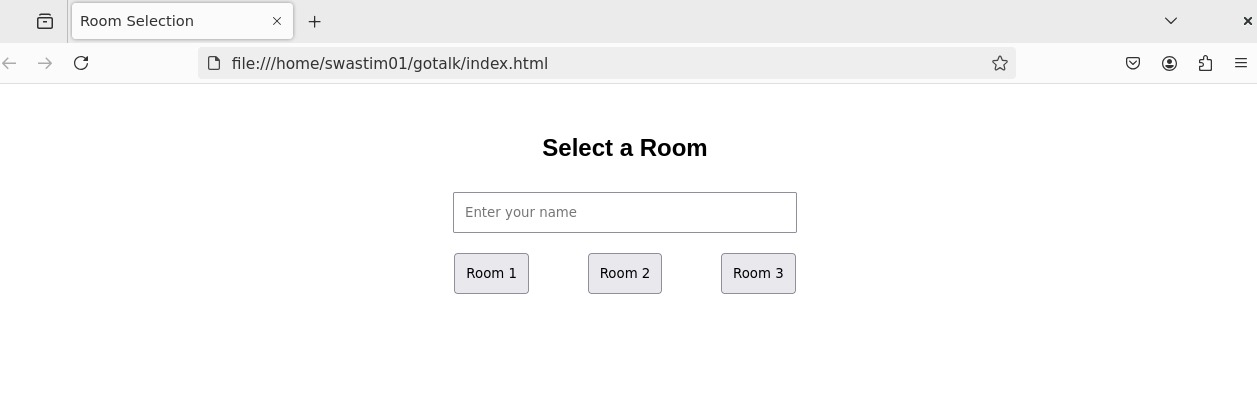
\includegraphics[width=\textwidth]{Pictures/room created.jpg}
        \end{minipage}
        \hfill
        \begin{minipage}[t]{0.5\textwidth}
            \centering
            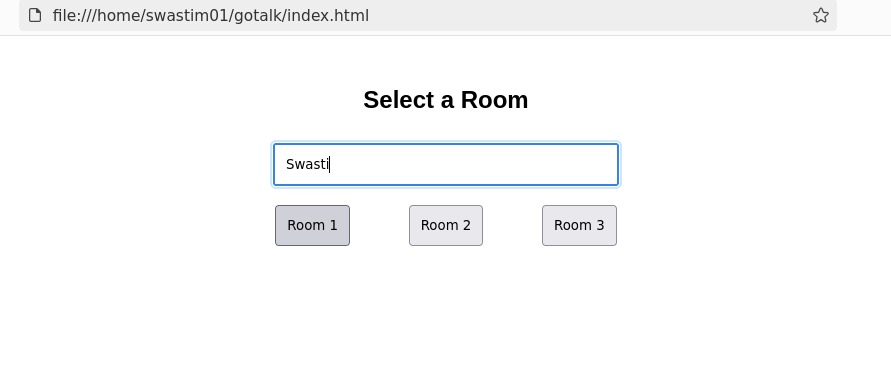
\includegraphics[width=\textwidth]{Pictures/nameinsertion.jpg}
        \end{minipage}
\end{frame}

\begin{frame}{Rooms Functionality}
        \begin{minipage}[t]{0.3\textwidth}
            \centering
            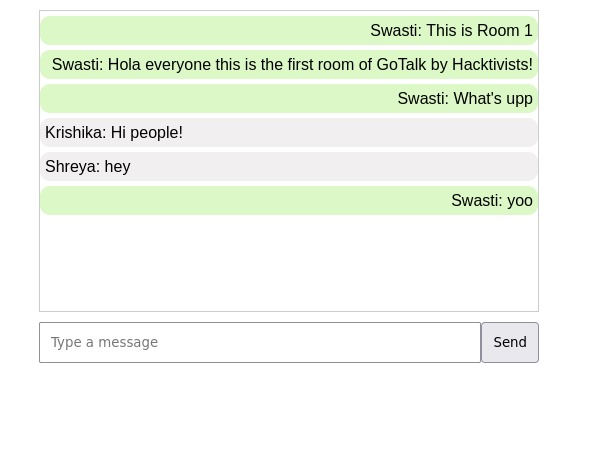
\includegraphics[width=\textwidth]{Pictures/room1.jpg}
        \end{minipage}
        \hfill
        \begin{minipage}[t]{0.3\textwidth}
            \centering
            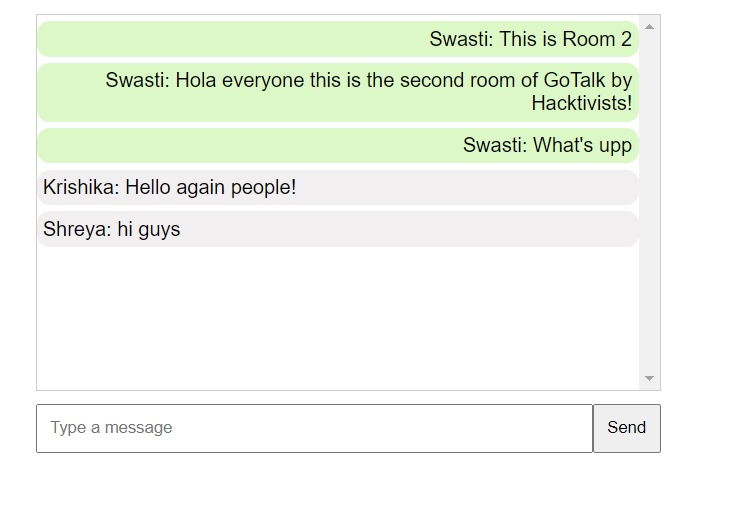
\includegraphics[width=\textwidth]{Pictures/room2.jpg}
        \end{minipage}
        \hfill
        \begin{minipage}[t]{0.3\textwidth}
            \centering
            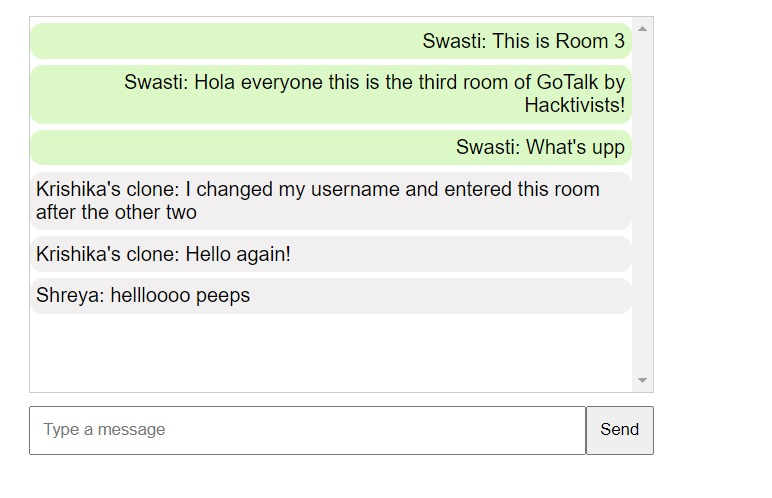
\includegraphics[width=\textwidth]{Pictures/room3.jpg}
        \end{minipage}
\end{frame}


\section{Conclusion}

\begin{frame}{Conclusion}
    \begin{itemize}
        \item Significant progress with real-time messaging, cookies and chat rooms.
        \item Upcoming enhancements for user experience.
    \end{itemize}
    \vfill
    \begin{center}
        \textbf{Thank you for your attention!}
    \end{center}
    \begin{center}
        Suggestions and Feedback welcomed.
    \end{center}
\end{frame}

\end{document}
